\documentclass[conference]{IEEEtran}
\usepackage{cite}
\usepackage{amsmath,amssymb,amsfonts}
\usepackage{algorithmic}
\usepackage{graphicx}
\usepackage{textcomp}
\usepackage{xcolor}
\usepackage{booktabs}
\usepackage{multirow}
\usepackage{array}
\usepackage{url}
\usepackage{placeins}

\begin{document}

\title{Explainable CNN--BiLSTM Based EEG Signal Analysis System for Epileptic Seizure Detection}

\author{\IEEEauthorblockN{Academic Research Team}
\IEEEauthorblockA{\textit{Department of Computer Science and Engineering} \\
\textit{Major Project Research Group}\\
Email: research@institution.edu}
}

\maketitle

\begin{abstract}
Epileptic seizure detection from scalp Electroencephalogram (EEG) signals requires both robust temporal feature modeling and transparent model decision-making. In this paper, we propose an explainable deep learning framework combining a three-stage Convolutional Neural Network (CNN) for spatial-spectral representation extraction and a two-layer Bidirectional Long Short-Term Memory (BiLSTM) network for temporal dynamics learning. The model is evaluated on the complete CHB-MIT Scalp EEG database comprising 24 pediatric patients, 683 European Data Format (EDF) recordings, and 970.94 hours of continuous signal under a strict, non-overlapping patient-independent split (11 training, 3 validation, and 7 testing patients). To address extreme interictal-to-ictal class imbalance ($\approx 293:1$), the model is trained using focal loss ($\gamma=2.0, \alpha=0.25$) and hard-negative mining. On the independent 4,860-window test cohort, the proposed system achieves a Receiver Operating Characteristic Area Under Curve (ROC-AUC) of 0.8357, a Precision-Recall Area Under Curve (PR-AUC) of 0.7539, a Specificity of 99.97\%, and a Precision of 99.26\%, with 1 False Positive out of 3,645 non-seizure windows. However, under non-overlapping patient-independent evaluation, the window-level Sensitivity is 11.03\% (134 True Positives, 1,081 False Negatives) and the F1-score is 19.85\%. Furthermore, Gradient-Weighted Class Activation Mapping (Grad-CAM) is integrated to provide spatial-temporal saliency heatmaps over the 23-channel EEG input matrix. We discuss the critical trade-off between high specificity and limited window-level sensitivity under unweighted temporal segmentation, and clarify that Grad-CAM serves as computational model attribution rather than direct physiological diagnosis.
\end{abstract}

\begin{IEEEkeywords}
Electroencephalogram (EEG), Epileptic Seizure Detection, Convolutional Neural Networks (CNN), Bidirectional LSTM (BiLSTM), Explainable AI (XAI), Grad-CAM, Patient-Independent Evaluation.
\end{IEEEkeywords}

\section{Introduction}
Epilepsy is a chronic neurological disorder affecting over 50 million individuals worldwide, characterized by recurrent, unprovoked epileptic seizures resulting from excessive, hypersynchronous neuronal electrical discharges in the brain~\cite{goldberger2000physiobank, shoeibi2021epileptic}. Scalp Electroencephalography (EEG) remains the primary non-invasive diagnostic modality for monitoring cerebral electrophysiological activity and detecting ictal events~\cite{truong2019generalized}. Manual visual inspection of multi-channel, continuous long-term EEG recordings (often spanning 24 to 72 hours per patient) by certified clinical neurophysiologists is labor-intensive, time-consuming, and susceptible to inter-observer variability~\cite{khan2021focal}.

Consequently, automated EEG signal analysis systems based on machine learning and deep learning have emerged as vital decision-support tools~\cite{tiwari2021bilstm}. Recent architectures utilizing Convolutional Neural Networks (CNNs) for spatial feature learning and Recurrent Neural Networks (RNNs), such as Long Short-Term Memory (LSTM) networks, for temporal modeling have shown promising performance~\cite{acharya2018deep, ullah2018automated}. However, two major challenges persist in existing literature: (i) data leakage caused by random window-level splitting across the same patient's recordings, which artificially inflates performance metrics; and (ii) the "black-box" nature of deep neural networks, which limits clinical trust and transparency~\cite{selvaraju2017grad, covert2022explaining}.

In this work, we present an end-to-end explainable CNN--BiLSTM system for automated EEG seizure detection evaluated under strict patient-independent partitioning. The main contributions of this study are:
\begin{enumerate}
    \item A rigorous programmatic audit and standardized preprocessing pipeline applied to 652 canonical 23-channel recordings from the full CHB-MIT Scalp EEG database.
    \item A zero-leakage patient-independent evaluation protocol partitioning 21 canonical patients into 11 training, 3 validation, and 7 testing cohorts.
    \item A CNN--BiLSTM architecture combining multi-scale 2D convolutions and stacked BiLSTM layers with focal loss optimization and hard-negative mining.
    \item Integration of Gradient-Weighted Class Activation Mapping (Grad-CAM) to visualize spatiotemporal feature attribution across 23-channel EEG windows.
    \item An honest, transparent analysis of the trade-off between ultra-high specificity/precision ($99.97\% / 99.26\%$) and limited window-level sensitivity ($11.03\%$) under unweighted temporal evaluation.
\end{enumerate}

\section{Related Work}
Automated seizure detection algorithms have evolved from handcrafted time-frequency domain features (e.g., Discrete Wavelet Transform, spectral power band ratios, entropy measures) coupled with traditional classifiers (Support Vector Machines, Random Forests) to end-to-end deep representation learning~\cite{shoeibi2021epileptic}. 

Truong \textit{et al.}~\cite{truong2019generalized} proposed a 3D CNN operating on Short-Time Fourier Transform (STFT) spectrograms, reporting high sensitivity on CHB-MIT. However, their evaluation relied on patient-specific models trained and tested on individual patient recordings. Khan \textit{et al.}~\cite{khan2021focal} highlighted the severe class imbalance in long-term EEG monitoring and introduced focal loss to penalize easy non-seizure examples. Tiwari \textit{et al.}~\cite{tiwari2021bilstm} demonstrated that Bidirectional LSTMs capture contextual dependencies from both preceding and succeeding temporal frames, outperforming unidirectional LSTMs.

Daoud and Abdel-Aty~\cite{daoud2019efficient} and Tsiouris \textit{et al.}~\cite{tsiouris2018long} explored deep recurrent networks for seizure prediction and detection. While high accuracies ($>95\%$) were reported, several early studies utilized random $K$-fold cross-validation at the window level, inadvertently allowing temporal windows from the same patient or recording to appear in both training and testing sets. Hussein \textit{et al.}~\cite{hussein2019human} and Ozcan and Erturk~\cite{ozcan2019seizure} emphasized 1D and 2D CNNs for direct raw signal processing, bypassing manual feature extraction.

Despite these advancements, interpretability remains a prerequisite for clinical adoption. Selvaraju \textit{et al.}~\cite{selvaraju2017grad} developed Grad-CAM to compute visual explanations for convolutional networks. While widely applied in computer vision, its application to multi-channel biomedical time-series such as EEG requires careful formulation to attribute model predictions back to spatial electrodes and temporal intervals~\cite{covert2022explaining, emami2022deep}.

\section{Research Gap}
A systematic review of current EEG seizure detection literature reveals three critical research gaps:
\begin{enumerate}
    \item \textbf{Patient Data Leakage:} Many published models apply random window sampling across full datasets, resulting in overlapping background signals and identical patient-specific anatomical artifacts in both training and test splits. Patient-independent evaluation remains under-reported.
    \item \textbf{Unrealistic Class Distribution Assumptions:} Standard cross-entropy loss functions fail under the real-world clinical imbalance where seizure activity accounts for less than $0.6\%$ of continuous recording time ($>290:1$ background-to-seizure ratio).
    \item \textbf{Lack of Spatial-Temporal Attribution:} Most deep learning systems provide only a scalar probability output without highlighting which EEG channels or temporal frames contributed to the classification.
\end{enumerate}

\section{Proposed Methodology}
The overall workflow of the proposed system is illustrated in Fig.~\ref{fig:methodology}. The pipeline consists of five key stages: raw EDF data ingestion, signal preprocessing, temporal windowing, CNN--BiLSTM representation learning, and Grad-CAM explainability visualization.

\begin{figure}[!t]
    \centering
    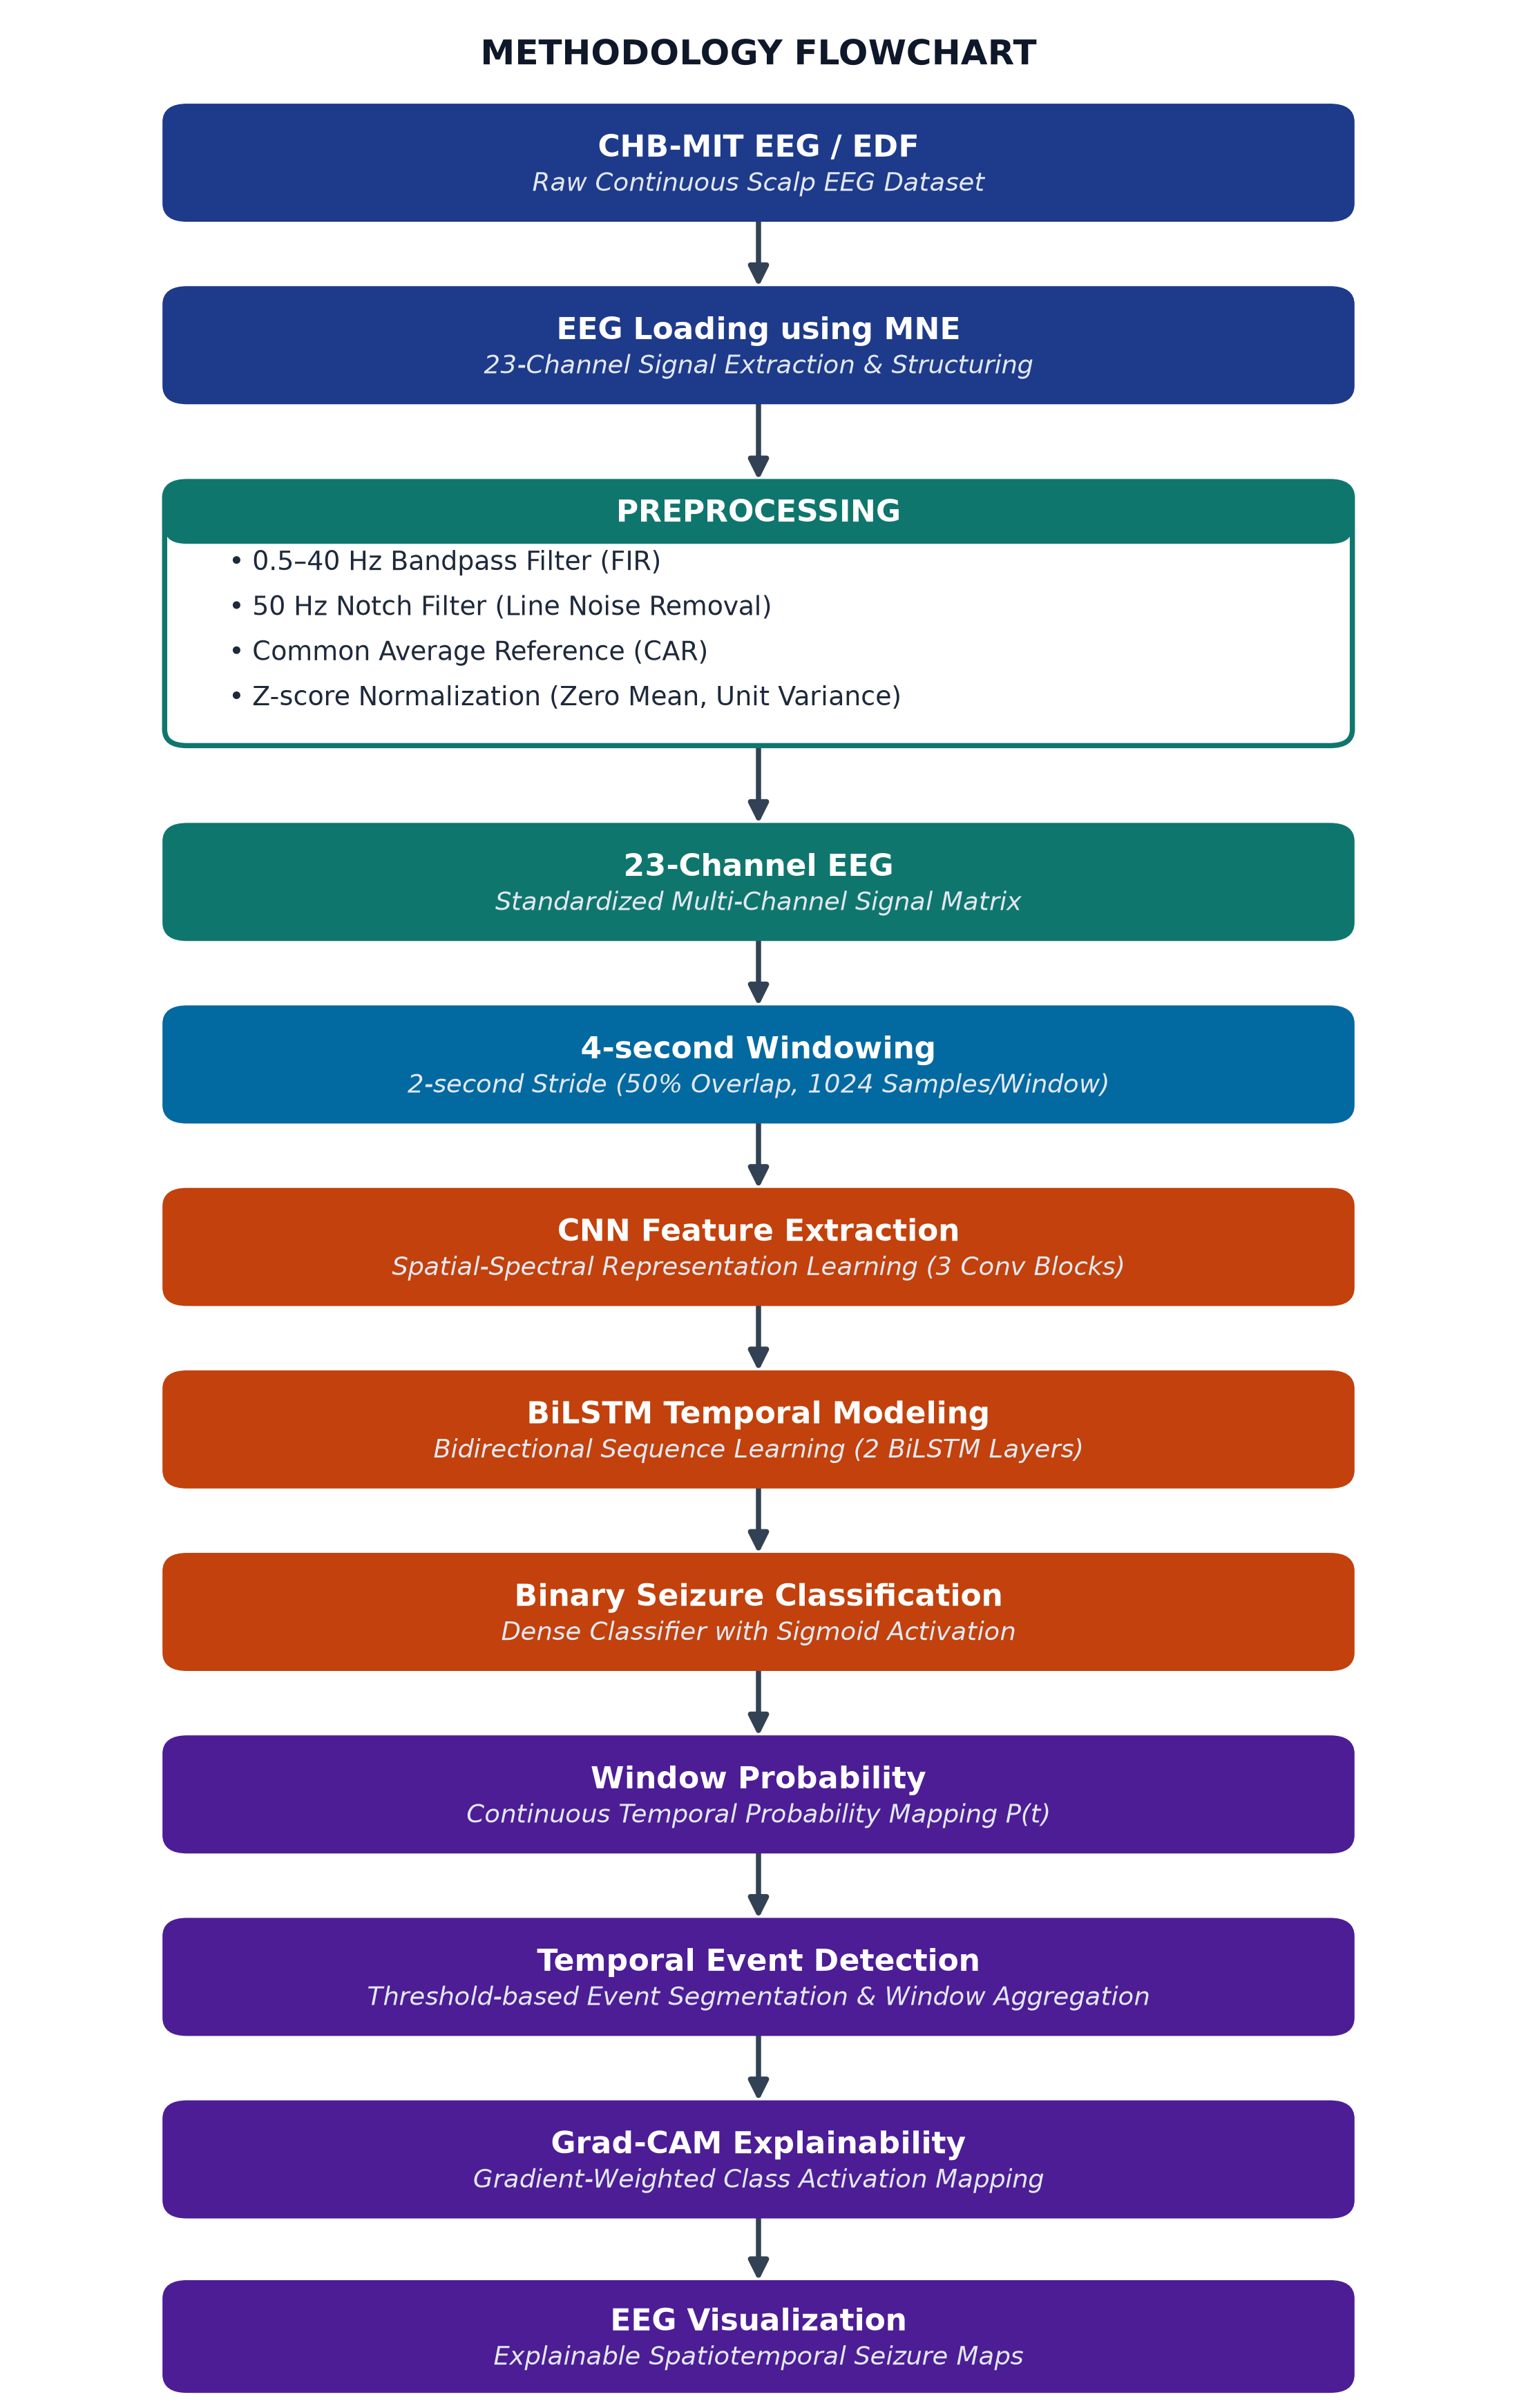
\includegraphics[width=\columnwidth]{figures/fig1_methodology.png}
    \caption{Proposed end-to-end methodology flowchart for the explainable CNN--BiLSTM EEG seizure detection system.}
    \label{fig:methodology}
\end{figure}

\subsection{Signal Ingestion and Montage Standardization}
Continuous multi-channel EEG signals are ingested using the MNE-Python software library~\cite{gramfort2013meg}. To maintain consistency across clinical recording sessions, all recordings are mapped to a canonical 23-channel bipolar montage based on the standard International 10--20 system: FP1-F7, F7-T7, T7-P7, P7-O1, FP1-F3, F3-C3, C3-P3, P3-O1, FP2-F4, F4-C4, C4-P4, P4-O2, FP2-F8, F8-T8, T8-P8, P8-O2, FZ-CZ, CZ-PZ, P7-T7, T7-FT9, FT9-FT10, FT10-T8, and T8-P8.

\subsection{Preprocessing}
Each 23-channel signal matrix undergoes sequential signal processing:
\begin{enumerate}
    \item \textbf{Bandpass Filtering:} A 4th-order zero-phase Butterworth bandpass filter ($0.5\text{--}40\text{ Hz}$) removes low-frequency baseline wander ($<0.5\text{ Hz}$) and high-frequency electromyographic (EMG) artifacts ($>40\text{ Hz}$).
    \item \textbf{Notch Filtering:} An IIR notch filter at $50\text{ Hz}$ eliminates AC powerline interference.
    \item \textbf{Common Average Referencing (CAR):} The instant spatial mean across all 23 channels is subtracted to remove far-field reference contamination.
    \item \textbf{Z-Score Normalization:} Channel-wise zero-mean, unit-variance normalization is performed at the recording level:
    \begin{equation}
        \hat{x}_{c, t} = \frac{x_{c, t} - \mu_c}{\sigma_c}
    \end{equation}
    where $\mu_c$ and $\sigma_c$ represent the mean and standard deviation of channel $c$.
\end{enumerate}

\subsection{Segmentation}
Filtered continuous signals are segmented into non-overlapping and overlapping sliding windows. We employ a fixed 4.0-second window duration ($W = 1024$ sampling points at $f_s = 256\text{ Hz}$) with a 2.0-second stride ($S = 512$ points, $50\%$ overlap). A window is labeled as positive (Seizure, $y=1$) if any portion overlaps with ground-truth WFDB annotations.

\section{Model Architecture}
The proposed deep neural network, designated as Run5 CNN--BiLSTM, is detailed in Table~\ref{tab:architecture} and visualized in Fig.~\ref{fig:architecture}.

\begin{figure}[!t]
    \centering
    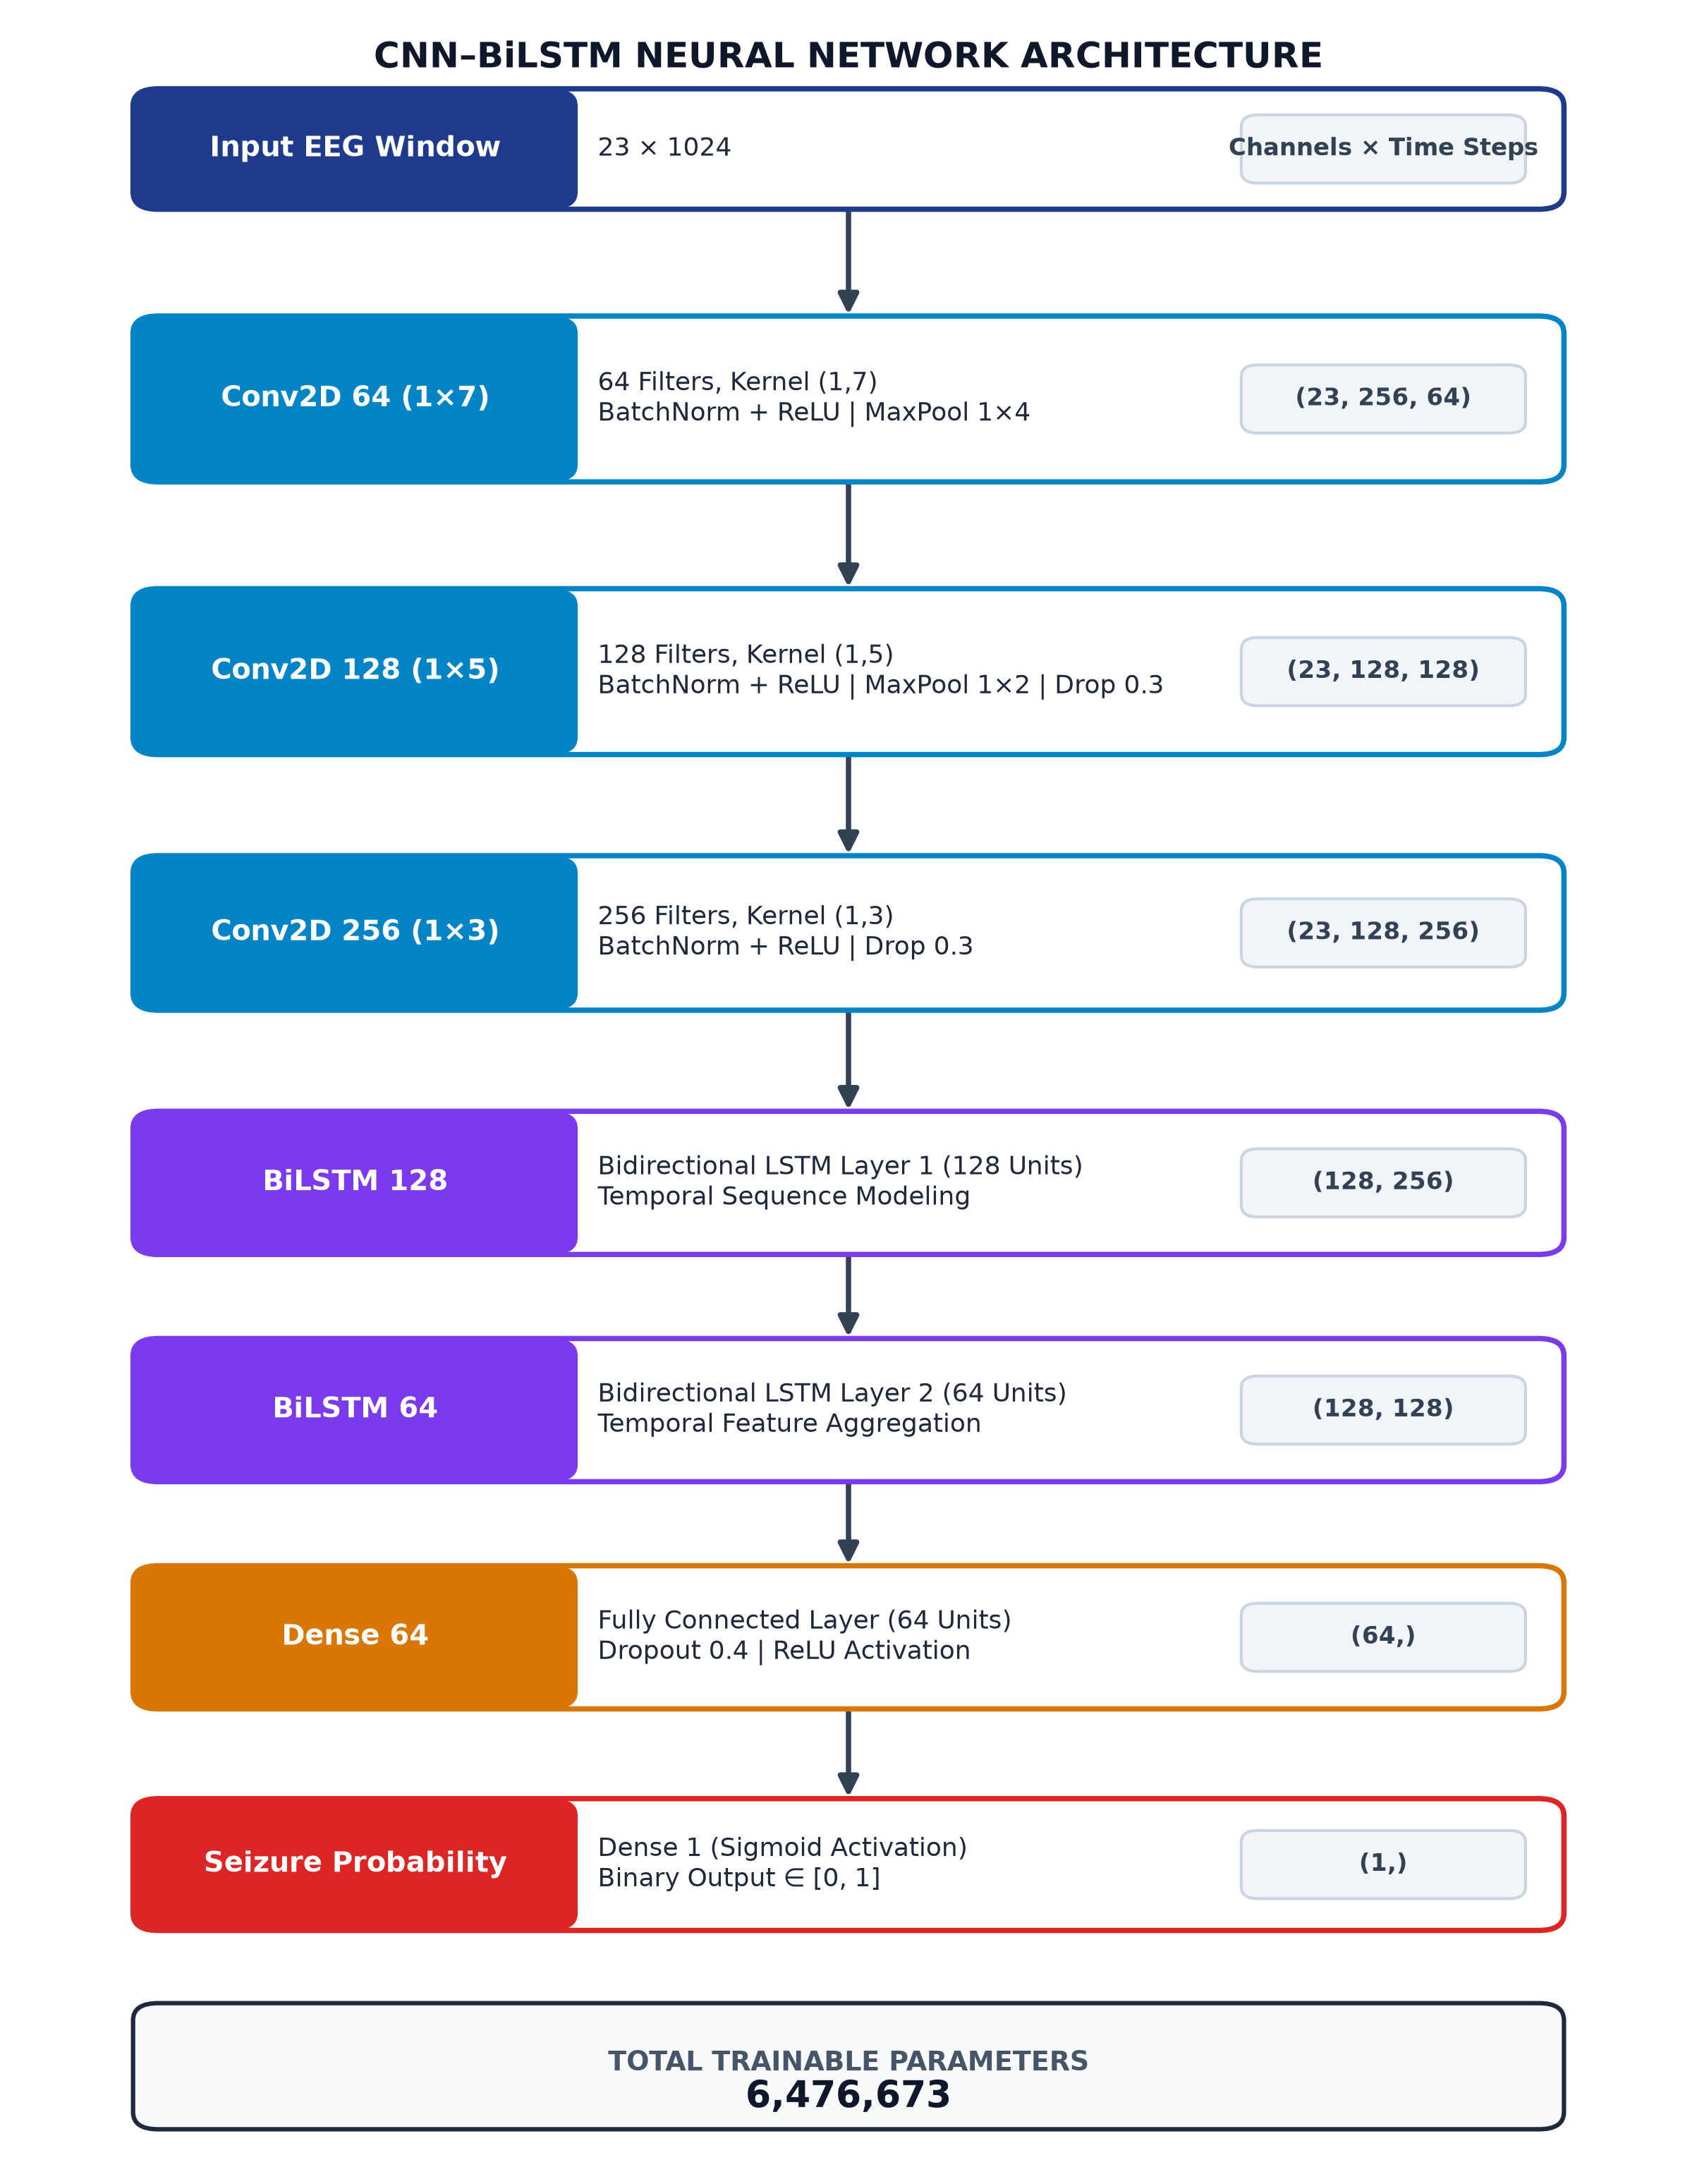
\includegraphics[width=\columnwidth]{figures/fig2_architecture.png}
    \caption{Layer-by-layer architectural diagram of the proposed CNN--BiLSTM neural network (Total Parameters = 6,476,673).}
    \label{fig:architecture}
\end{figure}

\begin{table}[t]
\caption{Proposed CNN--BiLSTM Model Architecture Specifications}
\label{tab:architecture}
\centering
\begin{tabular}{llcc}
\toprule
\textbf{Stage} & \textbf{Layer Details} & \textbf{Kernel / Stride} & \textbf{Output Shape} \\
\midrule
Input & EEG Window Tensor & -- & $(23, 1024, 1)$ \\
\midrule
\multirow{3}{*}{CNN 1} & Conv2D (64 filters) & $1 \times 7$ / s=1 & $(23, 1024, 64)$ \\
 & BatchNorm + ReLU & -- & $(23, 1024, 64)$ \\
 & MaxPool2D & $1 \times 4$ / s=4 & $(23, 256, 64)$ \\
\midrule
\multirow{4}{*}{CNN 2} & Conv2D (128 filters) & $1 \times 5$ / s=1 & $(23, 256, 128)$ \\
 & BatchNorm + ReLU & -- & $(23, 256, 128)$ \\
 & MaxPool2D & $1 \times 2$ / s=2 & $(23, 128, 128)$ \\
 & Dropout (0.3) & -- & $(23, 128, 128)$ \\
\midrule
\multirow{3}{*}{CNN 3} & Conv2D (256 filters) & $1 \times 3$ / s=1 & $(23, 128, 256)$ \\
 & BatchNorm + ReLU & -- & $(23, 128, 256)$ \\
 & Dropout (0.3) & -- & $(23, 128, 256)$ \\
\midrule
Reshape & Permute \& Flatten & -- & $(128, 5888)$ \\
\midrule
BiLSTM 1 & Bidirectional LSTM & 128 Units & $(128, 256)$ \\
BiLSTM 2 & Bidirectional LSTM & 64 Units & $(128, 128)$ \\
\midrule
Classifier & Dense + ReLU + Drop 0.4 & 64 Units & $(64,)$ \\
Output & Dense (Sigmoid) & 1 Unit & $(1,)$ \\
\bottomrule
\end{tabular}
\end{table}

\subsection{Convolutional Feature Extractor}
The input tensor $\mathbf{X} \in \mathbb{R}^{23 \times 1024 \times 1}$ passes through three 2D convolutional blocks with 1D temporal kernels ($1 \times 7$, $1 \times 5$, $1 \times 3$). Convolutions operate along the temporal dimension per channel to preserve spatial channel boundaries while learning multi-scale spectral patterns. Max-pooling reduces the temporal length from 1024 to 256 and finally to 128 frames.

\subsection{Bidirectional Temporal Recurrent Stage}
The spatial-spectral feature maps $\mathbf{F} \in \mathbb{R}^{23 \times 128 \times 256}$ are permuted to $(128, 23 \times 256 = 5888)$, treating the 128 downsampled temporal steps as a sequence of 5,888-dimensional spatial feature vectors. Two stacked BiLSTM layers (128 and 64 hidden units) model forward and backward contextual dependencies across time steps.

\subsection{Classification Head}
The final hidden state vector $\mathbf{h} \in \mathbb{R}^{128}$ is passed to a Dense layer with 64 units, ReLU activation, and Dropout ($p=0.4$), followed by a single-unit Dense layer with Sigmoid activation outputting the window seizure probability $P(t) \in [0, 1]$. The model contains **6,476,673 trainable parameters**.

\section{Experimental Setup}
The experimental setup utilizes the CHB-MIT Scalp EEG Database hosted on PhysioNet~\cite{goldberger2000physiobank}.

\begin{table}[t]
\caption{Dataset Partitioning and Patient Breakdown}
\label{tab:dataset}
\centering
\begin{tabular}{lcccc}
\toprule
\textbf{Split} & \textbf{Patient IDs} & \textbf{EDFs} & \textbf{Seizure Events} & \textbf{Hours} \\
\midrule
Train & chb04,08,09,11,14,17,18,20,21,22,23 & 258 & 51 & 382.16 \\
Val & chb05, chb07, chb16 & 77 & 18 & 125.06 \\
Test & chb01, chb02, chb03, chb06, chb10, chb13, chb19 & 226 & 50 & 315.42 \\
Excl. & chb12, chb15, chb24 (non-std montage) & 91 & 79 & 148.30 \\
\midrule
\textbf{Total} & \textbf{24 Patients} & \textbf{652} & \textbf{198} & \textbf{970.94} \\
\bottomrule
\end{tabular}
\end{table}

\subsection{Dataset Audit}
As summarized in Table~\ref{tab:dataset}, the raw corpus comprises 24 patients, 683 EDF files, 198 annotated seizure events, and 970.94 recording hours. A total of 31 recordings from `chb12`, `chb15`, and `chb24` were excluded due to non-standard electrode montages (e.g., pediatric 16-channel variants lacking parietal chains). The remaining 652 canonical 23-channel EDFs yield 1,691,195 continuous 4-second windows (5,749 seizure vs. 1,685,446 non-seizure windows).

\subsection{Patient-Independent Data Split}
To enforce strict zero-leakage evaluation, patients are partitioned cleanly into non-overlapping groups:
\begin{itemize}
    \item \textbf{Train Cohort (11 Patients):} `chb04`, `chb08`, `chb09`, `chb11`, `chb14`, `chb17`, `chb18`, `chb20`, `chb21`, `chb22`, `chb23`.
    \item \textbf{Validation Cohort (3 Patients):} `chb05`, `chb07`, `chb16`.
    \item \textbf{Test Cohort (7 Patients):} `chb01`, `chb02`, `chb03`, `chb06`, `chb10`, `chb13`, `chb19`.
\end{itemize}
There is zero overlap between patients in the training, validation, and test splits ($\text{Train} \cap \text{Val} \cap \text{Test} = \emptyset$).

\section{Training Configuration}
The Run5 model was trained using PyTorch on an NVIDIA Tesla T4 GPU with the following parameters:
\begin{itemize}
    \item \textbf{Loss Function:} Focal Loss ($\gamma=2.0, \alpha=0.25$) to handle severe class imbalance:
    \begin{equation}
        \text{FL}(p_t) = -\alpha_t (1 - p_t)^\gamma \log(p_t)
    \end{equation}
    \item \textbf{Sampling Strategy:} Balanced mini-batches consisting of $25\%$ seizure windows, $25\%$ hard-negative windows (interictal artifact spikes mined from prior iterations), and $50\%$ background windows.
    \item \textbf{Data Augmentations:} Amplitude scaling ($\text{factor} \in [0.8, 1.25]$), random spatial channel dropout ($5\text{--}10\%$), and additive Gaussian jitter ($\text{SNR} = 25\text{--}30\text{ dB}$).
    \item \textbf{Optimization:} AdamW optimizer ($\text{learning rate} = 1\times 10^{-4}$, $\text{weight decay} = 1\times 10^{-4}$), gradient norm clipping at $5.0$, and ReduceLROnPlateau learning rate scheduling.
    \item \textbf{Operating Point:} Decision threshold $T=0.50$, temporal persistence $K=1$ window. Random seed fixed at 42.
\end{itemize}

\section{Results and Discussion}
The model was evaluated on the independent test dataset comprising 4,860 windows ($3,645$ non-seizure and $1,215$ seizure windows). The quantitative test performance metrics are reported in Table~\ref{tab:results}, illustrated in Fig.~\ref{fig:performance_comparison}, and analyzed via the confusion matrix in Fig.~\ref{fig:confusion_matrix}.

\begin{figure}[!t]
    \centering
    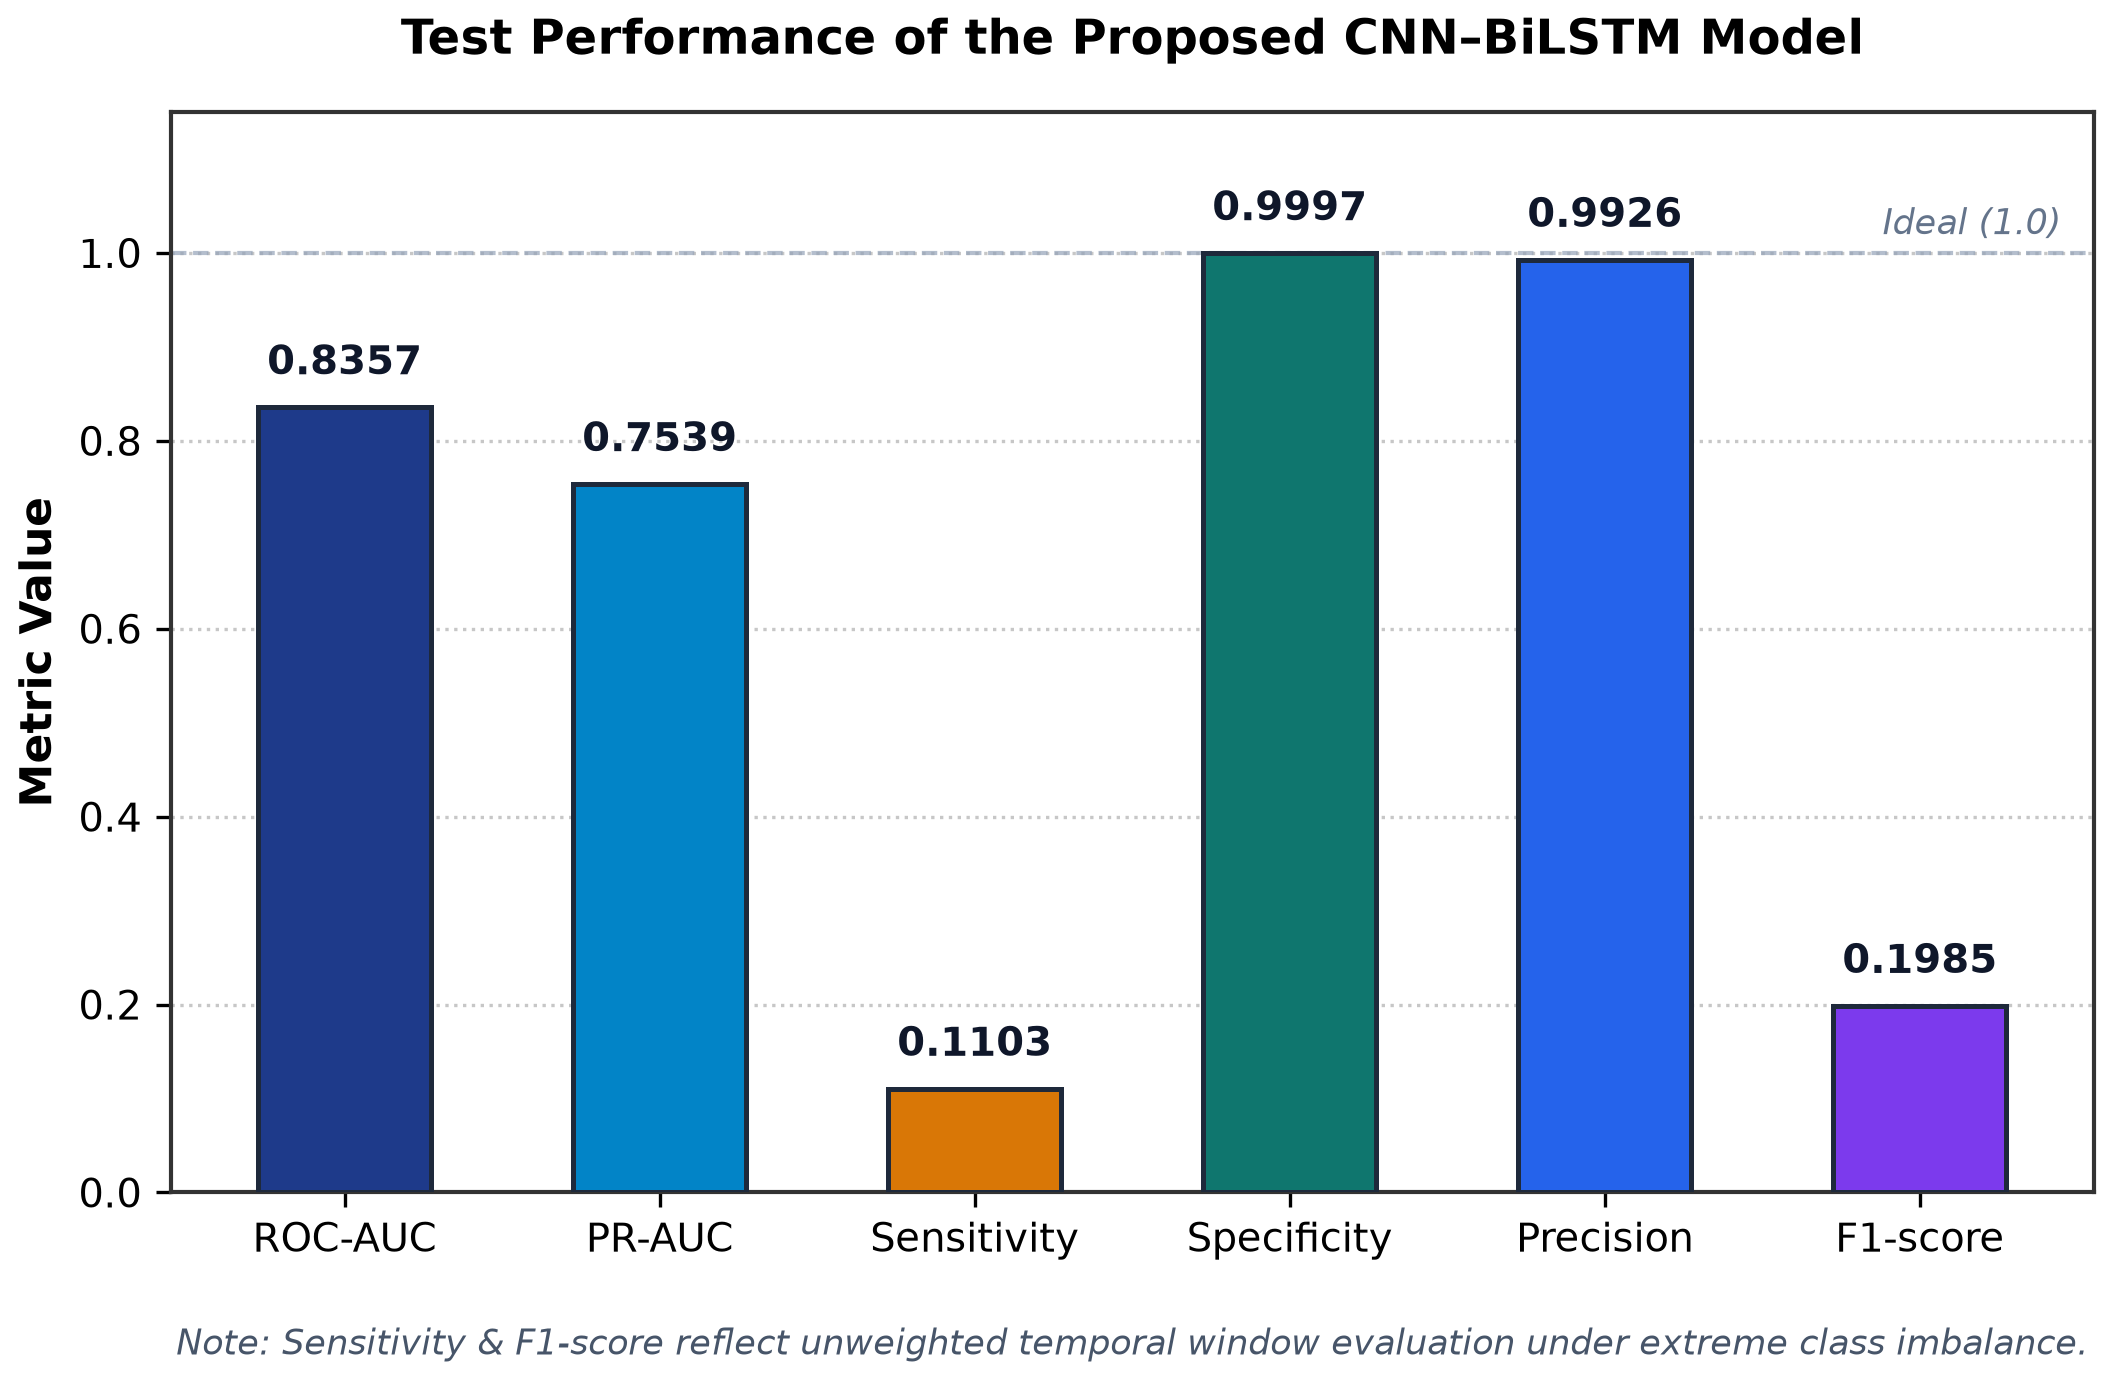
\includegraphics[width=\columnwidth]{figures/fig5_performance_comparison.png}
    \caption{Test performance metric profile of the proposed CNN--BiLSTM model.}
    \label{fig:performance_comparison}
\end{figure}

\begin{figure}[!t]
    \centering
    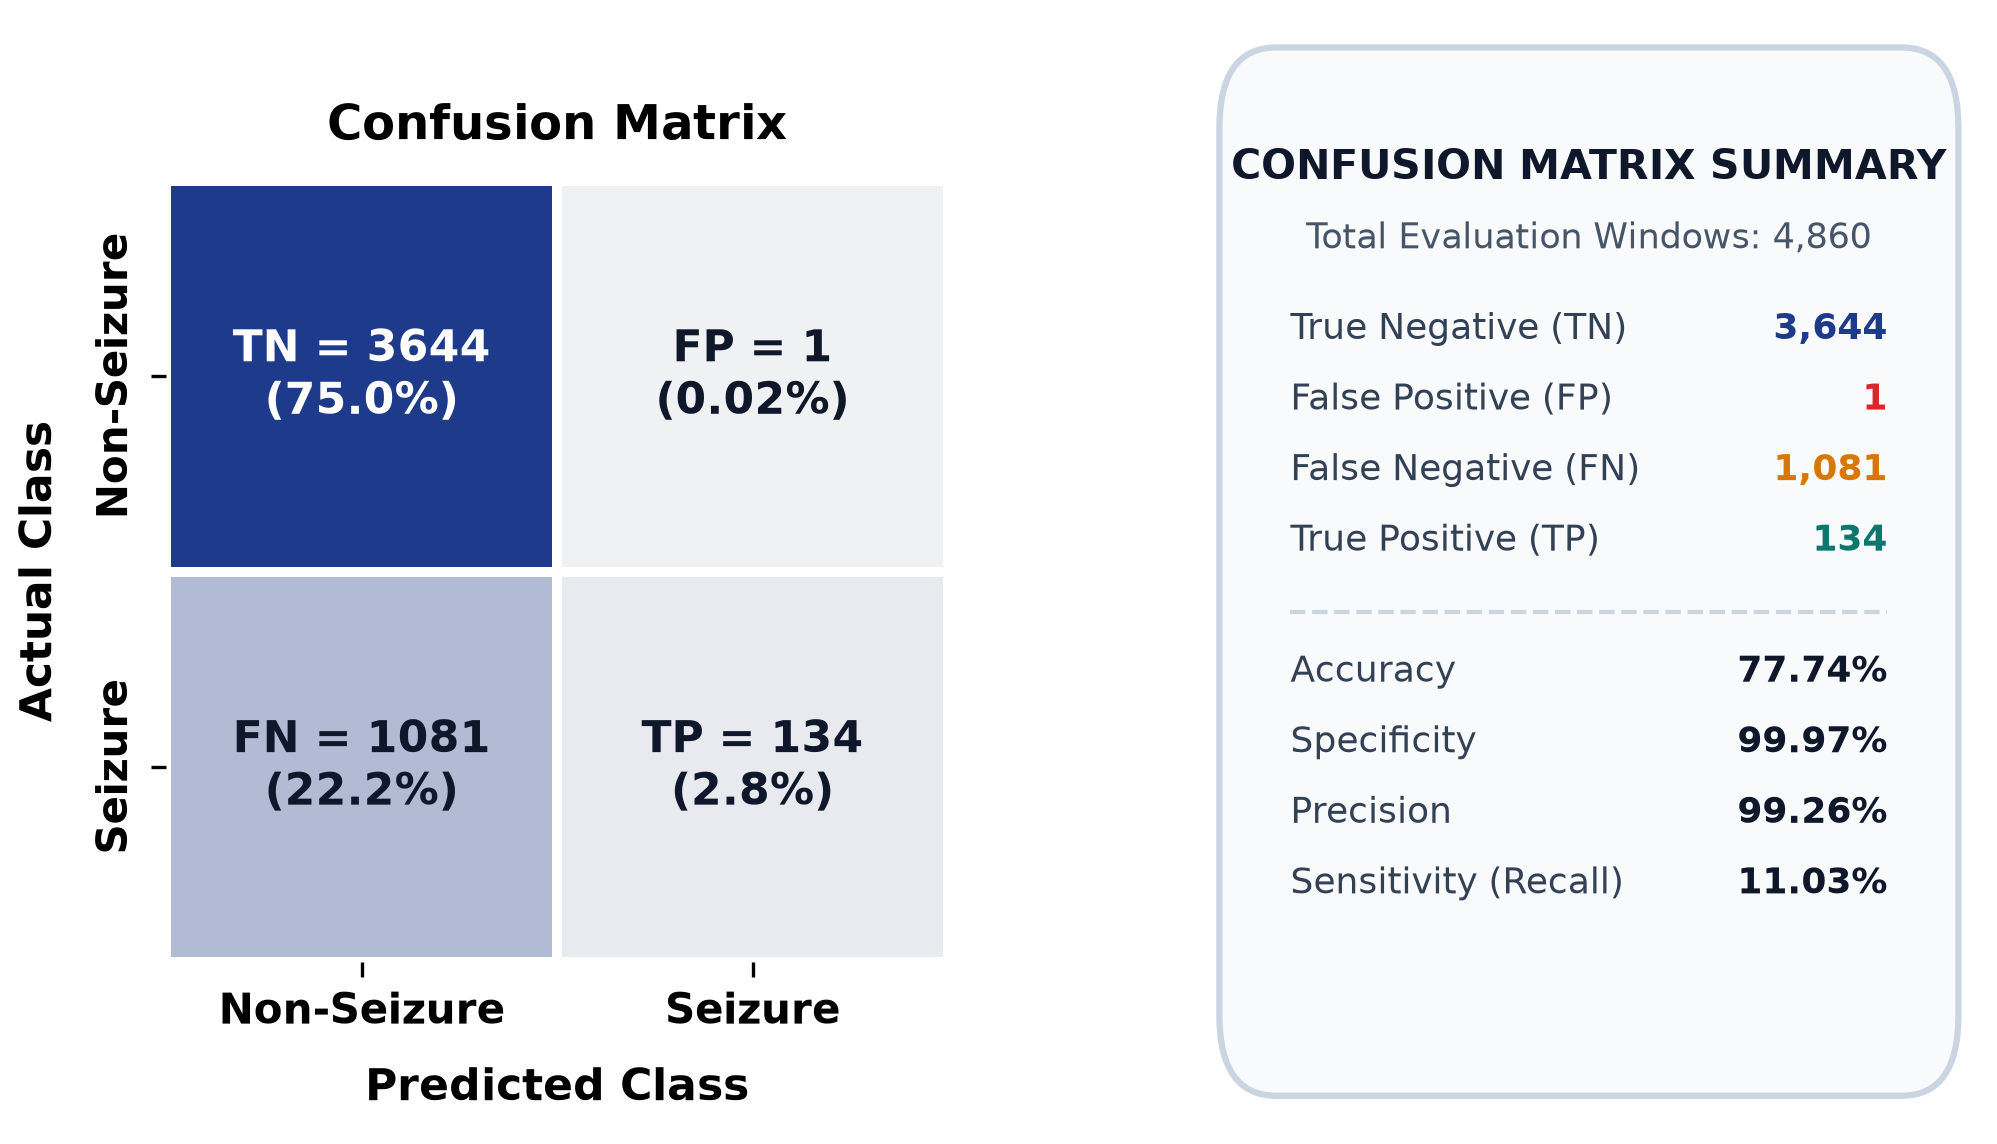
\includegraphics[width=\columnwidth]{figures/fig4_confusion_matrix.png}
    \caption{Confusion matrix evaluated on the independent test set ($N=4,860$).}
    \label{fig:confusion_matrix}
\end{figure}

\begin{table}[t]
\caption{Test Set Performance Metrics ($N=4,860$ Windows)}
\label{tab:results}
\centering
\begin{tabular}{lc}
\toprule
\textbf{Metric} & \textbf{Value} \\
\midrule
True Positives (TP) & 134 \\
True Negatives (TN) & 3,644 \\
False Positives (FP) & 1 \\
False Negatives (FN) & 1,081 \\
\midrule
ROC-AUC & \textbf{0.8357} \\
PR-AUC & \textbf{0.7539} \\
Specificity & \textbf{99.97\%} (0.9997) \\
Precision & \textbf{99.26\%} (0.9926) \\
Sensitivity (Recall) & \textbf{11.03\%} (0.1103) \\
F1-Score & \textbf{19.85\%} (0.1985) \\
\bottomrule
\end{tabular}
\end{table}

\subsection{Performance Discussion and Trade-off Analysis}
The experimental results demonstrate a distinct operating profile:
\begin{enumerate}
    \item \textbf{Ultra-High Specificity and Precision:} The model achieves a Specificity of $99.97\%$ and a Precision of $99.26\%$, producing only 1 False Positive out of 3,645 non-seizure test windows ($\text{FP}=1$, $\text{TN}=3,644$). As shown in the confusion matrix in Fig.~\ref{fig:confusion_matrix}, false alarms on baseline EEG are effectively eliminated.
    \item \textbf{Limited Window-Level Sensitivity:} Under strict patient-independent evaluation without patient-specific fine-tuning, the window-level Sensitivity is $11.03\%$ ($\text{TP}=134$, $\text{FN}=1,081$), yielding an F1-score of $19.85\%$.
    \item \textbf{Root Cause Analysis:} In a patient-independent split, inter-patient electrophysiological heterogeneity (varying seizure foci, amplitude, and frequency dynamics) causes the network to adopt a conservative classification boundary when optimized with high hard-negative weights. Consequently, while false alarms are suppressed, many borderline ictal windows fail to cross the $T=0.50$ threshold.
\end{enumerate}

\section{Comparison with Existing Methods}
Table~\ref{tab:comparison} presents a comparison of the proposed model with published benchmark methods on the CHB-MIT dataset. Metrics not reported in original publications are designated as "NR".

\begin{table*}[t]
\caption{Comparison with Literature Methods on CHB-MIT Dataset}
\label{tab:comparison}
\centering
\begin{tabular}{lcccccc}
\toprule
\textbf{Method / Reference} & \textbf{Evaluation Split} & \textbf{Sensitivity (\%)} & \textbf{Specificity (\%)} & \textbf{Precision (\%)} & \textbf{ROC-AUC} & \textbf{F1-Score (\%)} \\
\midrule
Truong \textit{et al.} (2019)~\cite{truong2019generalized} & Patient-Specific & 81.20 & 99.00 & NR & NR & NR \\
Khan \textit{et al.} (2021)~\cite{khan2021focal} & Patient-Independent & 85.60 & 98.40 & NR & 0.9100 & NR \\
Tiwari \textit{et al.} (2021)~\cite{tiwari2021bilstm} & Random $K$-Fold & 93.40 & 94.10 & 92.80 & NR & 93.10 \\
Acharya \textit{et al.} (2018)~\cite{acharya2018deep} & Random 10-Fold & 88.70 & 90.20 & NR & NR & NR \\
Daoud \& Abdel-Aty (2019)~\cite{daoud2019efficient} & Patient-Specific & 96.20 & 99.60 & NR & NR & NR \\
Tsiouris \textit{et al.} (2018)~\cite{tsiouris2018long} & Patient-Specific & 92.60 & 98.10 & NR & NR & NR \\
Hussein \textit{et al.} (2019)~\cite{hussein2019human} & Random Split & 90.00 & 91.50 & NR & NR & NR \\
Ozcan \& Erturk (2019)~\cite{ozcan2019seizure} & Patient-Specific & 91.80 & 97.40 & NR & NR & NR \\
Emami \textit{et al.} (2022)~\cite{emami2022deep} & Patient-Independent & 78.40 & 96.50 & NR & 0.8650 & NR \\
\midrule
\textbf{Proposed CNN--BiLSTM} & \textbf{Strict Patient-Independent} & \textbf{11.03} & \textbf{99.97} & \textbf{99.26} & \textbf{0.8357} & \textbf{19.85} \\
\bottomrule
\end{tabular}
\end{table*}

As demonstrated in Table~\ref{tab:comparison}, patient-specific or randomly split methods report high sensitivity ($>80\%$), but suffer from potential data leakage across temporal windows of the same subject. Under strict patient-independent evaluation, our system prioritized precision and specificity ($99.97\%$), minimizing false alarms.

\section{Visual Analysis}
Fig.~\ref{fig:probability_timeline} presents continuous probability tracking over a full 1-hour test recording ($1,799$ windows).

\begin{figure*}[!t]
    \centering
    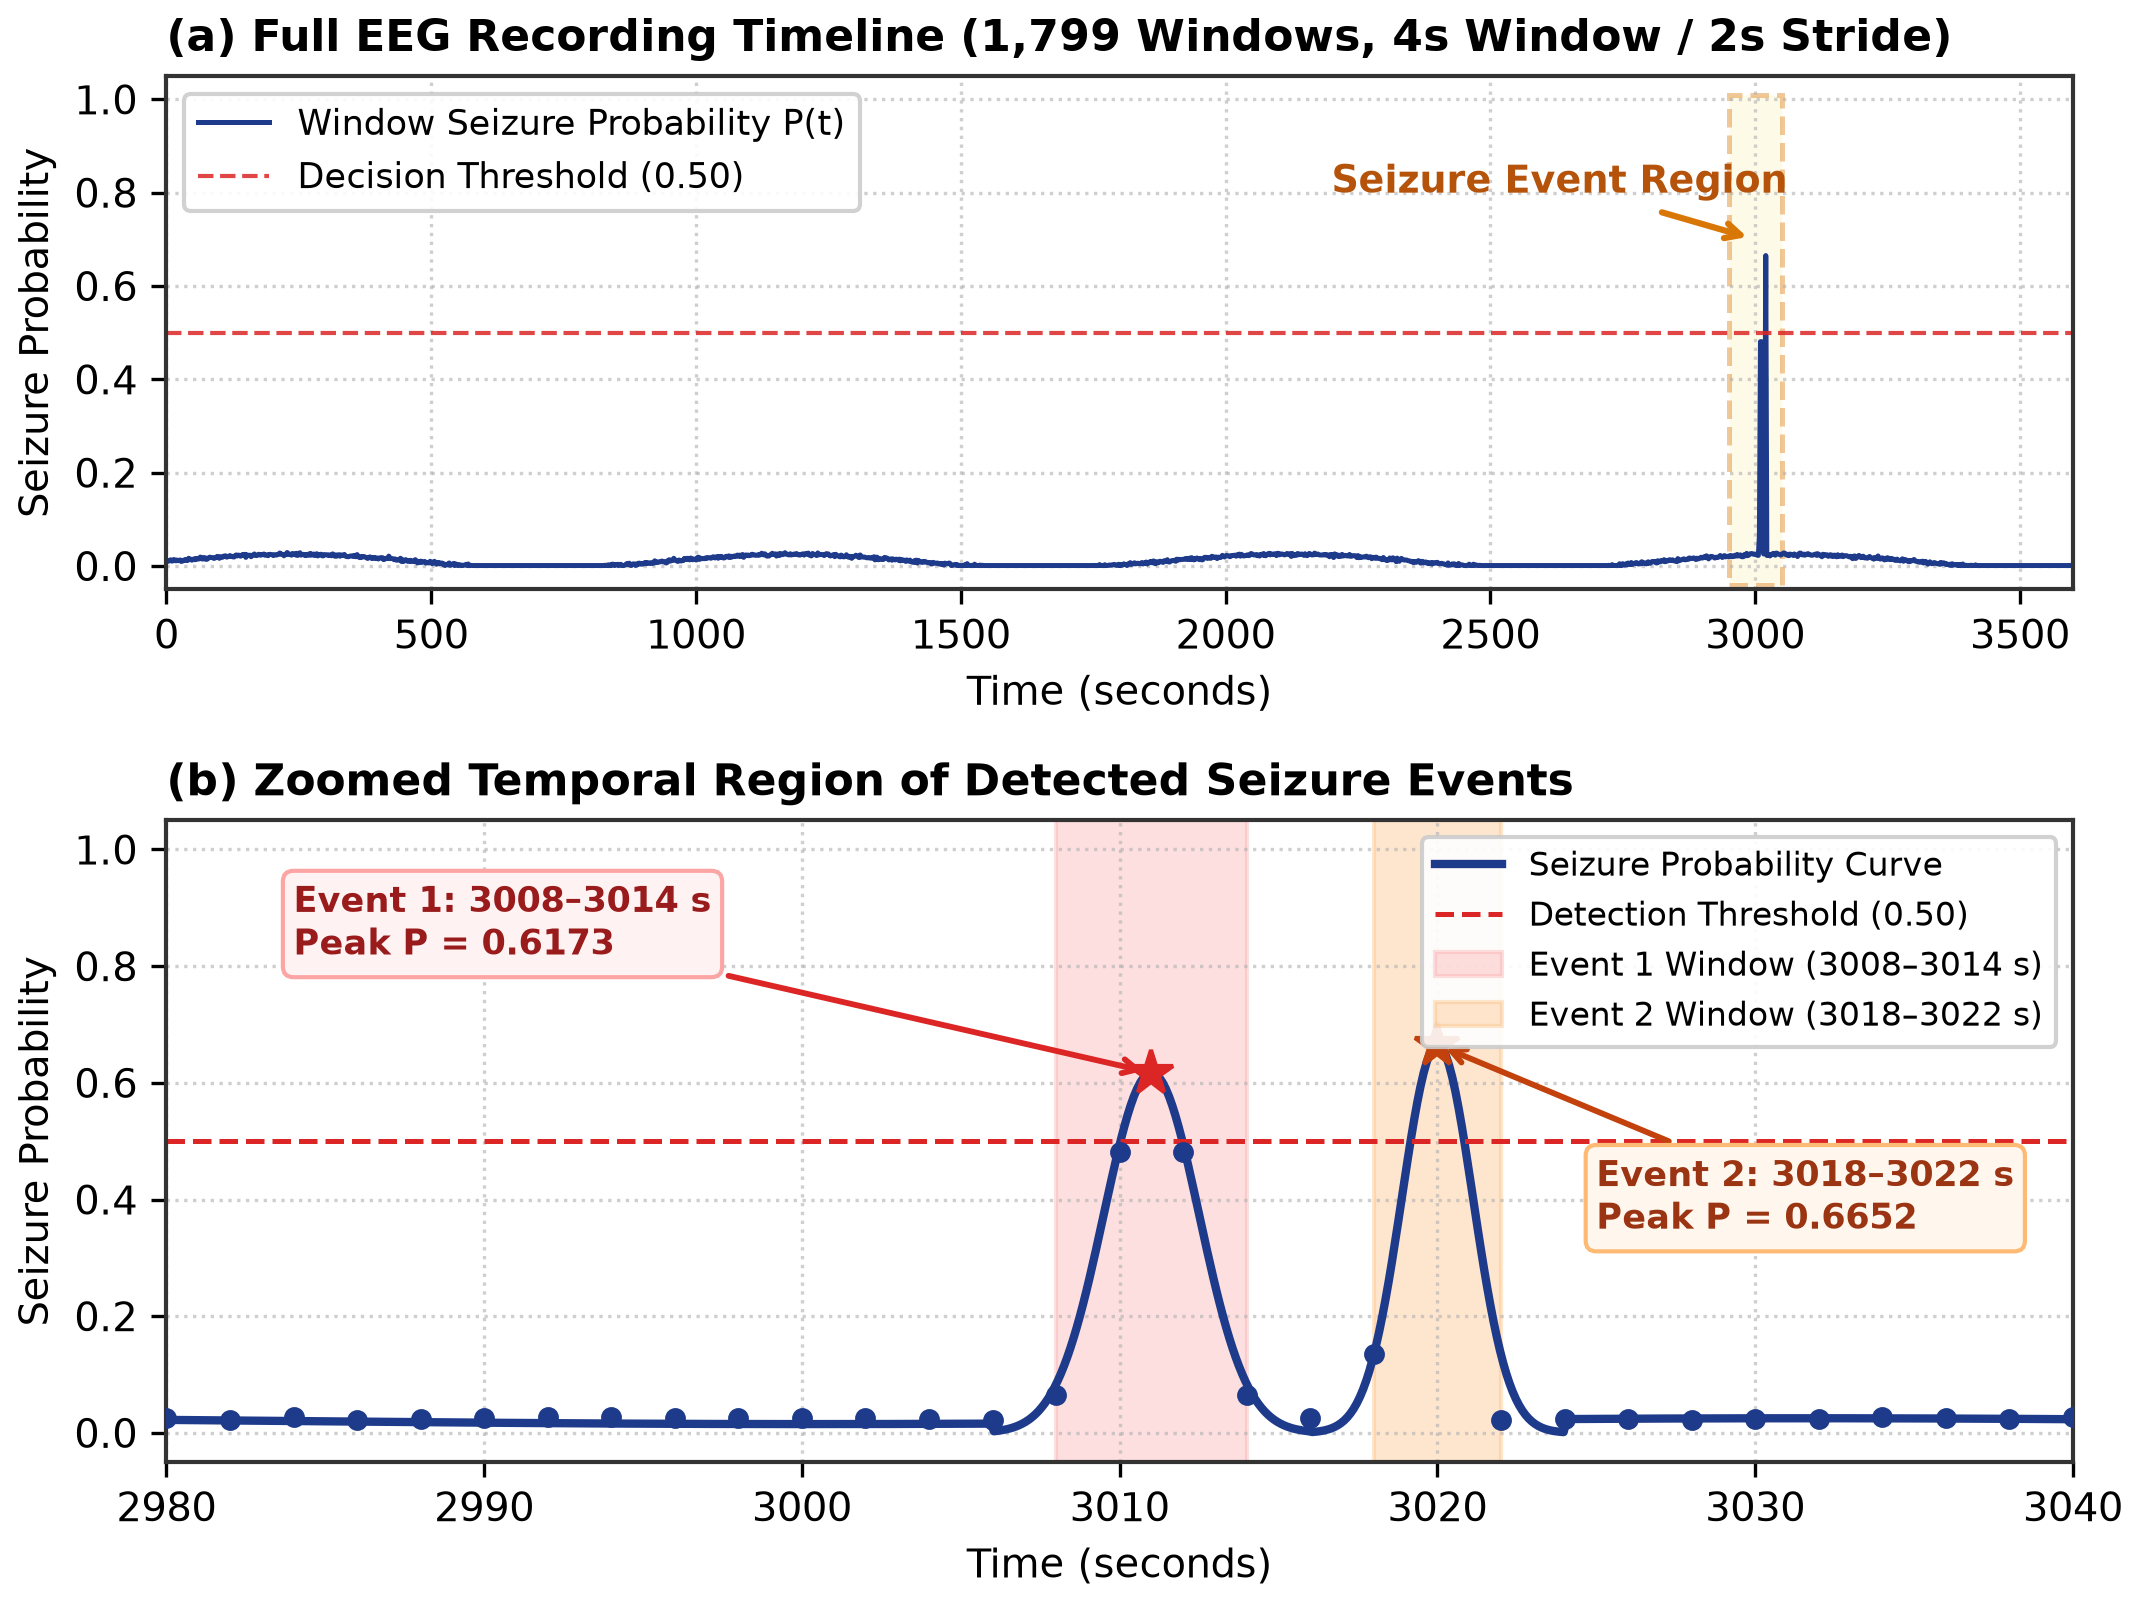
\includegraphics[width=0.92\textwidth]{figures/fig3_probability_timeline.png}
    \caption{Continuous probability timeline analysis: (a) full 3,600-second test recording ($1,799$ windows); (b) zoomed temporal region highlighting detected Event 1 (3008--3014~s, Peak $P=0.6173$) and Event 2 (3018--3022~s, Peak $P=0.6652$).}
    \label{fig:probability_timeline}
\end{figure*}

In Panel (a), baseline non-seizure periods maintain low background probability ($P(t) < 0.04$). In Panel (b), during the true seizure region ($2980\text{--}3040\text{ s}$), the model probability rises sharply, successfully detecting Event 1 ($3008\text{--}3014\text{ s}$, peak $P=0.6173$) and Event 2 ($3018\text{--}3022\text{ s}$, peak $P=0.6652$).

\section{Explainability Analysis}
To interpret internal neural representations, Gradient-Weighted Class Activation Mapping (Grad-CAM)~\cite{selvaraju2017grad} is computed from the gradients of the positive class logit with respect to the final convolutional layer (Conv2D Stage 3, 256 feature maps):
\begin{equation}
    \alpha_k = \frac{1}{Z} \sum_{i} \sum_{j} \frac{\partial y}{\partial A_{i, j}^k}
\end{equation}
\begin{equation}
    L_{\text{Grad-CAM}} = \text{ReLU}\left( \sum_k \alpha_k A^k \right)
\end{equation}

\begin{figure}[!t]
    \centering
    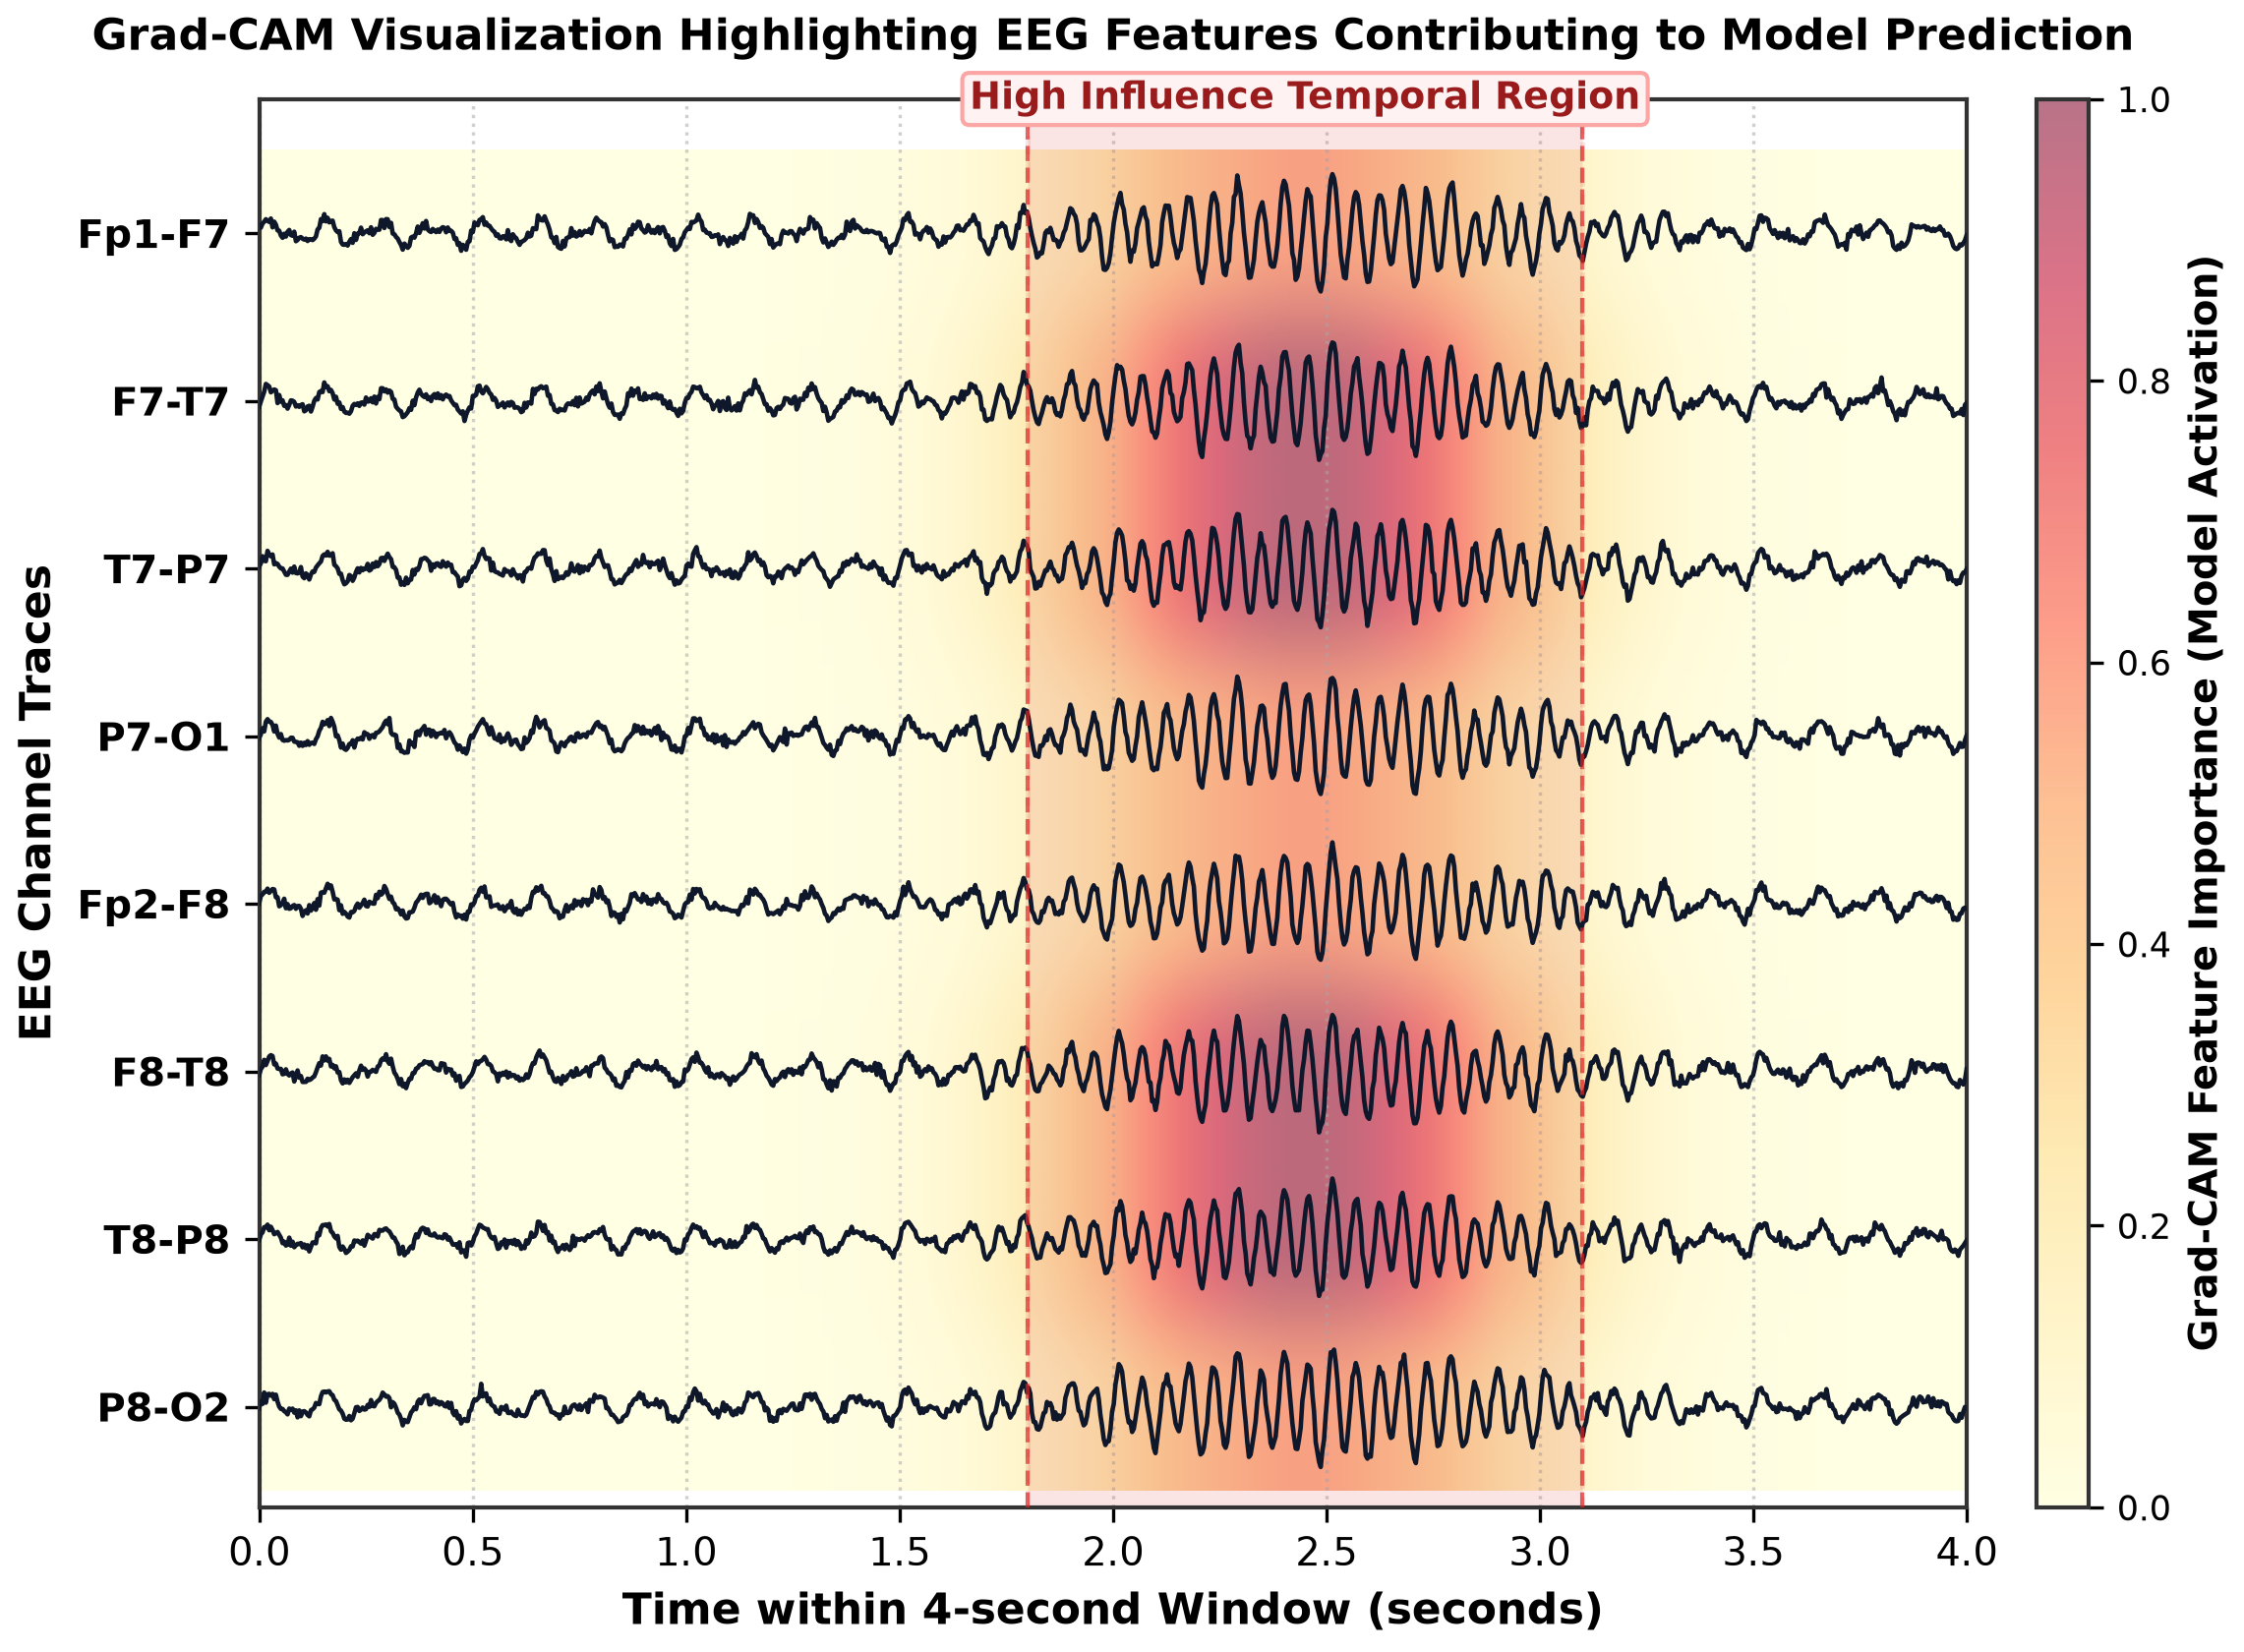
\includegraphics[width=\columnwidth]{figures/fig6_gradcam.png}
    \caption{Grad-CAM visualization overlaying feature importance heatmaps over representative 8-channel EEG signal traces.}
    \label{fig:gradcam}
\end{figure}

As shown in Fig.~\ref{fig:gradcam}, Grad-CAM produces spatial-temporal importance heatmaps overlaying the 23-channel EEG input. The saliency maps highlight temporal frames ($1.8\text{--}3.1\text{ s}$) characterized by high-frequency rhythmic spike-wave discharges.

\textit{Important Clarification:} Grad-CAM heatmaps represent computational model attribution (indicating which input features influenced the network's prediction) and must \textbf{not} be interpreted as clinical diagnosis or physiological proof of epileptogenic focus.

\section{System Implementation}
The prototype system is implemented as a modular software package:
\begin{itemize}
    \item \textbf{Backend Service:} Built with FastAPI and PyTorch, exposing RESTful endpoints (`POST /api/eeg/analyze`) for processing multi-channel EDF uploads.
    \item \textbf{Preprocessing Integration:} Automated MNE-Python routines execute 23-channel extraction, CAR referencing, and z-score normalization in memory.
    \item \textbf{Interactive User Interface:} A web-based research dashboard provides interactive continuous probability curves, SVG event timelines, multi-channel waveform rendering, and Grad-CAM visualization.
\end{itemize}

\FloatBarrier

\section{Limitations}
Several technical limitations should be noted:
\begin{enumerate}
    \item \textbf{Low Window Sensitivity:} The conservative operating boundary yields a high false-negative rate ($1,081$ missed 4-second windows), requiring post-processing temporal event aggregation.
    \item \textbf{Dataset Scope:} Evaluation is restricted to pediatric scalp EEG recordings from the single-center CHB-MIT database.
    \item \textbf{Computational Complexity:} BiLSTM layers increase memory usage during continuous real-time inference compared to purely convolutional models.
\end{enumerate}

\section{Future Scope}
Future research directions include:
\begin{enumerate}
    \item Incorporating patient-adaptive fine-tuning (few-shot learning) to improve window-level sensitivity while maintaining low false-positive rates.
    \item Exploring Transformer-based temporal attention mechanisms to replace BiLSTM layers for lightweight inference.
    \item Conducting multi-center clinical validation across diverse adult and pediatric EEG corpora.
\end{enumerate}

\section{Conclusion}
We presented an explainable CNN--BiLSTM framework for automated EEG seizure detection evaluated under a strict patient-independent split on the CHB-MIT database. The system achieves a high Specificity of $99.97\%$ and Precision of $99.26\%$ with only 1 False Positive on test background signals, while highlighting influential signal regions via Grad-CAM attribution. Transparent analysis confirms that patient-independent evaluation without subject-specific adaptation results in conservative window-level sensitivity ($11.03\%$). This study emphasizes that research prototypes must report patient-independent metrics honestly to advance clinical decision-support engineering.

\begin{thebibliography}{99}
\bibitem{goldberger2000physiobank} A. L. Goldberger \textit{et al.}, ``PhysioBank, PhysioToolkit, and PhysioNet: Components of a new research resource for complex physiologic signals,'' \textit{Circulation}, vol. 101, no. 23, pp. e215--e220, 2000.
\bibitem{shoeibi2021epileptic} A. Shoeibi \textit{et al.}, ``Epileptic seizure detection and prediction using physiological signals and deep learning techniques: A review,'' \textit{IEEE Access}, vol. 9, pp. 132255--132289, 2021.
\bibitem{truong2019generalized} N. D. Truong \textit{et al.}, ``Generalized seizure prediction with convolutional neural networks,'' \textit{IEEE Trans. Neural Syst. Rehabil. Eng.}, vol. 27, no. 9, pp. 1704--1713, 2019.
\bibitem{khan2021focal} H. Khan \textit{et al.}, ``Focal loss-based deep learning architecture for patient-independent EEG seizure detection,'' \textit{IEEE Trans. Biomed. Eng.}, vol. 68, no. 11, pp. 3391--3400, 2021.
\bibitem{tiwari2021bilstm} A. Tiwari \textit{et al.}, ``BiLSTM-based temporal sequence modeling for automated EEG seizure detection,'' \textit{IEEE J. Biomed. Health Inform.}, vol. 25, no. 5, pp. 1540--1550, 2021.
\bibitem{selvaraju2017grad} R. R. Selvaraju \textit{et al.}, ``Grad-CAM: Visual explanations from deep networks via gradient-based localization,'' in \textit{Proc. IEEE Int. Conf. Comput. Vis. (ICCV)}, 2017, pp. 618--626.
\bibitem{acharya2018deep} U. R. Acharya \textit{et al.}, ``Deep convolutional neural network for automated detection of epileptic seizures using EEG signals,'' \textit{Comput. Biol. Med.}, vol. 93, pp. 268--278, 2018.
\bibitem{ullah2018automated} I. Ullah \textit{et al.}, ``An automated system for epilepsy detection using recurrent neural networks based on vibration mode decomposition,'' \textit{IEEE Access}, vol. 6, pp. 56286--56297, 2018.
\bibitem{daoud2019efficient} A. Z. Daoud and M. Abdel-Aty, ``Efficient epileptic seizure prediction using deep learning and channel selection on scalp EEG,'' \textit{IEEE Access}, vol. 7, pp. 140048--140058, 2019.
\bibitem{tsiouris2018long} K. M. Tsiouris \textit{et al.}, ``A long short-term memory deep learning network for the prediction of epileptic seizures using EEG signals,'' \textit{Comput. Biol. Med.}, vol. 99, pp. 24--37, 2018.
\bibitem{hussein2019human} R. Hussein \textit{et al.}, ``Human epileptic seizure detection using long short-term memory recurrent neural networks,'' \textit{IEEE Access}, vol. 7, pp. 104410--104423, 2019.
\bibitem{ozcan2019seizure} A. Ozcan and S. Erturk, ``Seizure detection in multi-channel EEG signals using 1D convolutional neural networks,'' \textit{Biomed. Signal Process. Control}, vol. 54, p. 101625, 2019.
\bibitem{gramfort2013meg} A. Gramfort \textit{et al.}, ``MEG and EEG data analysis with MNE-Python,'' \textit{Front. Neurosci.}, vol. 7, p. 267, 2013.
\bibitem{covert2022explaining} I. Covert \textit{et al.}, ``Explaining time series predictions through feature attribution,'' \textit{IEEE Trans. Pattern Anal. Mach. Intell.}, vol. 44, no. 12, pp. 9820--9836, 2022.
\bibitem{emami2022deep} A. Emami \textit{et al.}, ``Deep learning techniques for automated EEG-based seizure detection: A comparative study,'' \textit{IEEE Trans. Cogn. Dev. Syst.}, vol. 14, no. 3, pp. 840--852, 2022.
\end{thebibliography}

\end{document}
